%%%%%%%%%%%%%%%%%%%%%%%%%%%%%%%%%%%%%%%%%%%%%%%%%%%%%%%%%%%%%%%%%%%%
%% LaTeX Template Version 2.3
%%
%% Nathan Lowrie
%% The Widget Foundry
%%
%% (C)2007 - Free for personal use, please email me improvements to
%% solodex2151@gmail.com
%%%%%%%%%%%%%%%%%%%%%%%%%%%%%%%%%%%%%%%%%%%%%%%%%%%%%%%%%%%%%%%%%%%%

% Preamble
    % Packages included
    \documentclass[letterpaper,10pt]{RevisedBook}
    \usepackage{ifthen}
    \usepackage[ansinew]{inputenc}
%     \usepackage{graphics}
    \usepackage{fancyhdr}
    \usepackage{amsmath}	
     \usepackage[final]{graphicx}
     \usepackage{supertabular}
    
    \oddsidemargin 0in
    \evensidemargin 0in
    \textwidth 6.5in
    
    \pagestyle{fancy}
    \sloppy
    \nonfrenchspacing
    \renewcommand{\baselinestretch}{1.0}
    \clubpenalty=9999    % Not higher!
    \widowpenalty=9999   % Not higher!
    \setcounter{secnumdepth}{4}
    \setcounter{tocdepth}{3}
%    \makeindex
    \addtolength{\skip\footins}{5mm}

% Some custom macros
    % Titlerule is a FAT ruler
    \newcommand{\titlerule}{\rule{\linewidth}{1.5mm}}

    % For comments in the draft - work in progress
    \newcommand{\betainsert}[2]{\fbox{#1}\marginnote{\textsf{#2}}}

    % Notes in the margin are nicer this way.
    \newcommand{\marginnote}[1]{\marginpar{\scriptsize\raggedright #1}}

% Do you want to have the possibility of including color in your PDFs?
    \usepackage{color}

% Check if in PDFLaTeX or ``normal''
    \newif\ifpdf
      \ifx\pdfoutput\undefined
      \pdffalse
    \else
      \pdfoutput=1
      \pdftrue
    \fi

%Define variables
\renewcommand{\title}{The Dabo Book}				%Title Goes Here
\newcommand{\subtitle}{3-Tier Applications Made Easy}	%Subtitle Goes Here
\renewcommand{\author}{Paul McNett, Nathan Lowrie}					%Author Goes Here
\newcommand{\copyrightHolder}{Ed Leafe, Paul McNett, et. al.}	%Copyright Holder Goes Here
\newcommand{\subject}{3-tier desktop applications}					%Subject Goes Here
\newcommand{\keywords}{Dabo, Python, database}					%Keywords go here
    
% Set up PDF specific. These are used when the file is compiled with 
% pdflatex instead of ordinary latex.
    \ifpdf
      % if PDFLaTeX use these parameters
      \usepackage[pdftex,colorlinks=true,urlcolor=blue,pdfstartview=FitH]{hyperref}
      \pdfcompresslevel=9
      \hypersetup{
			pdftitle={\title},			%Enter title here
			pdfauthor={\author},				%Enter Author here
			pdfsubject={\subject},		%Enter Subject here
			pdfkeywords={\keywords}		%Enter Keywords here
      } 
    \else
      % Ordinary tex use these parameters
      \usepackage{hyperref}
    \fi
   
\begin{document}

\frontmatter									% only in book class (roman page #s)

% Making a nice TITLEPAGE
\begin{titlepage}
    \thispagestyle{empty}
    \begin{center}
%    \includegraphics[width= 8cm]{logo}			%Uncomment if you want a logo graphic
    \end{center}
    \vspace*{\stretch{1}}
    \begin{center}
        \titlerule\\[3mm]
        \Huge \textsc{\title\\\subtitle}\\[5mm]		%Enter Title and subtitle here
        \begin{center}
		\huge \author\\[3.5mm]						%Enter company or person authoring
    	\end{center}
       	\titlerule\\
    \end{center}
    \scriptsize \today
    \vspace*{\stretch{2}}
    \begin{center}
        \textcopyright 2004-2007 \copyrightHolder			%Enter company or person for copyright here
    \end{center}
\end{titlepage}

\pagestyle{fancy}                         %Forces the page to use the fancy template

% Setting up pagestyles for ``fancy''
\setlength\headheight{23.11pt}
\renewcommand{\chaptermark}[1]{\markboth{\emph{#1}}{}}%\textbf{Chapter \thechapter}:\ \emph{#1}}{}}
\renewcommand{\sectionmark}[1]{\markright{\thesection\ \boldmath\textbf{#1}\unboldmath}}
                                          %The text used in the header is determined by the arguments to the \markboth
                                          % and \markright commands used here. The chapter information will appear as the
                                          % chapter number in bold, followed by a dot and a space, followed by the chapter
                                          % title (dealt with by LaTeX---no user intervention needed here) in italics. The
                                          % section information will appear as the section number, followed by a space, and
                                          % then the section title (again generated automatically) in bold. Any maths in
                                          % the section title will also appear in bold (provided the bold font exists).
\fancyhf{}                                %Clears all header and footer fields, in preparation.
\fancyhead[LO, RE]{\textbf{\title}\\\textbf{\subtitle}}
                                          %Displays the Title and subtitle the header,
                                          % to the left on odd pages and to the right on even pages.
\fancyhead[LE, RO]{\nouppercase{\leftmark}}   %Displays the upper-level (chapter) information---
                                          % as determined above---in non-upper case in the header, to the left on even pages.
						                  %Displays the lower-level (section) information---as
                                          % determined above---in the header, to the right on odd pages.
% \fancyfoot[c]{\textcopyright\ 2004-2007 \copyrightHolder}
\fancyfoot[LE,RO]{\thepage}
\fancyfoot[LO,RE]{\today}
\renewcommand{\headrulewidth}{1.3pt}      %Underlines the header. (Set to 0pt if not required).
\renewcommand{\footrulewidth}{1.3pt}      %Underlines the footer. (Set to 0pt if not required).

\tableofcontents
\listoffigures
\listoftables
\newpage

% --- DOCUMENT START ---


% Preface for the dabo book

\chapter{Preface}

Microsoft purchased Fox Software and gained the knowledge base to produce the 
best user-friendly application development suites in the industry. Using Visual Basic, 
Access, .NET, COM, MSDE and FoxPro, hundreds of thousands of developers and 
consultants world-wide were able to provide solutions for their clients, from 
shrink-wrapped applications to completely custom programs.

For over a decade, the situation was mutually beneficial: the large company got to 
make billions off its operating system, and the developer got to make a living selling 
solutions using low-priced development tools provided by that same large company.

Something started happening, however, late in the 1990's. At a time when everyone 
thought Unix was uttering its final words, "Linux" became a household term. A 
student's hobby in 1991 became a world-class enterprise operating system by 1998, 
and since then Linux has made impressive gains in the user application space: the 
desktop. At about the same time, Apple Computer released Darwin - another Unix 
based operating system - to the open source world and built a rock-solid user 
friendly interface on top of it, and today Apple's successful future seems guaranteed: 
elegant, user-friendly applications built on top of Darwin/OS X, such as iTunes, 
iPhoto, iDVD, and iMovie are reverberating among a growing user base.

A sea change is underway. Up until now, and into 2006, the open source community 
has been playing catch-up with Microsoft, trying to make applications that do 
everything the typical Microsoft Windows user expects, in the same ubiquitous 
fashion. As I type this (September 2004) I can say that the open source community 
has almost caught up. OpenOffice.org is approaching version 2.0, and can already 
replace Microsoft Office for all but the most complex Word, Powerpoint, and Excel 
documents. Mozilla Firefox and Thunderbird are approaching 1.0, and already 
handle browsing and emailing better than Microsoft Internet Explorer and Outlook. 
The Gnome and KDE Linux desktops, besides being fast and stable, now have all 
the goodies any modern user would want. From now on, the catch-up phase is over, 
and real innovation will begin to be defined not by one huge company, but by a 
loosely-knit community of open source developers from all over the world. The big 
company will have to become a part of that community - and play by its rules - or 
risk being sucked into the undertow.

We aren't quite there yet. One very important missing piece for software development 
on Linux or Mac is a comprehensive, easy-to-use, flexible Integrated Development 
Environment (IDE), such as Microsoft Visual Basic, that lets people develop powerful 
applications without necessarily having to know how to write great code. An IDE is 
basically a collection of power tools, such as a visual form designer, a graphical 
debugger, a project manager, and a help system. Until such an application becomes 
available, the only people developing open source applications will be people 
comfortable with the command line, make files, and a c compiler.

Enter Dabo, an open source, data aware, 3-tier development framework that you 
can use to develop open source and/or proprietary applications for distribution to 
your customers. Dabo aims to be easy to learn, fun to work with, flexible, and 
powerful. You can program in Python by hand using any editor, or you can use the 
Dabo IDE which centralizes all the files in your project and offers all the power tools 
you need to create your databases, build your user interface, write your business 
rules, and create your reports (printouts or previews of your data, formatted the 
way you define).

%Not really sure what this is so I commented it out.
%Intro paragraph - first paragraph style

\section{Target Audience}

The Dabo Book assumes some knowledge of a typical Microsoft-like IDE such as 
Visual Basic or Visual FoxPro, but that isn't required to get by. All that is really 
needed is the desire to create a killer application. Follow along with the examples, 
and you'll know all you need to know in no time at all.

If you happen to have experience with the Python programming language, which 
Dabo is built on top of, that is great but again not required.

In a nutshell, this book is for anyone wishing to develop a desktop application that 
will run on Linux, Macintosh, and Windows, and that will connect to an external 
database to get and store data.

\section{Organization of this Book}

The book is organized into several parts:

\subsection{Context and Introduction}

Covers the history of Dabo as well as its features, architecture, components, and 
install methods. Also includes an introduction to the Python programming language.

\subsection{Dabo Overview and Patterns}

Explains the components that make up Dabo, shows some simple examples, 
introduces the new user to the Python language, and goes into some detail on the 
"Three Tiers of Dabo". Also shows the typical structure of a Dabo application, and 
the typical workflow patterns of creating a Dabo application.

\subsection{Tutorials}

Here is where the fun begins. Follow along with the design and implementation of a 
"real-world" data-aware application, from start to finish. From the structure of the
database, to the writing of the business rules, to the designing of the screens and 
application framework, to debugging and documenting, to source control, this is the 
real meat of the book. Get through this and you'll know how to start making your 
own application.

\subsection{API Reference}

You won't necessarily want to read this part of the book from beginning to end, 
but it'll probably be well thumbed through, as it'll be your reference to all the 
properties, methods, and events available for your use while developing your 
application.

\subsection{Appendices}

A number of stand-alone articles are presented here, including an in-depth tour of 
the Dabo Report Designer, debugging tactics, visual design options, how to contribute 
to the development of Dabo, and more.


\fancyhead[RO]{Chapter \thechapter}

\mainmatter                             % only in book class (arabic page #s)
\newpage

%Put your parts and chapters here
% Will house all of the introduction components
% Each chapter gets it's own file

\part{Introduction}

%What is dabo chapter

\chapter{What is Dabo?}

Dabo provides an abstraction layer for a variety of open source projects, for the 
purpose of providing a solid and flexible framework for developing multiplatform 
data-aware business applications. User/developers can use the powerful Python 
programming language to write their business logic and lay out their user-interface 
elements, harnessing the Dabo framework and thus not getting preoccupied with the 
implementation details.

\section{3-Tier}

Dabo provides a 3-tier approach to application design, separating database access 
from business rules from user-interface layout. Dabo also provides an Application 
object that provides common functions and controls the event loop.

Dabo allows you to use each tier independently, for instance only using the database 
tier for a simple script, or only using the UI tier for a simple GUI app that doesn't 
need database access. But those use-cases will be limited. In a typical Dabo 
application, 90\% of the user code will end up in the business tier, using subclasses 
of dBizobj, 0\% in the database tier, and the rest as layout code 
in the user-interface tier.

Dabo's tiers are related in a chain-of-responsibility pattern, so that when a user 
chooses, for example, to save their changes, the user-interface will communicate 
that request to the business object, which will validate the request against the 
business rules, and if all rules pass the request will go to the database tier to 
actually save the change to the database. If the change fails, such as in the 
business object for validation reasons, or in the database tier for connectivity 
reasons, the exception gets propagated back up to the user-interface tier and the 
user is notified.

\section{Flexible Database Support}

Dabo supports all databases for which there is a Python wrapper that conforms to 
the dbapi version 2. This includes MySQL, PostgreSQL, SQLite, Firebird, and 
Microsoft SQL Server. 

\section{Flexible User Interface Support}

After version 1.0, Dabo will support a selection of user-interface libraries, as 
illustrated in (need fig-tier3-1). The support of multiple libraries while allowing the 
Dabo developer to use a common API makes Dabo a very flexible, powerful solution. 
Different toolkits have their pros and cons; you can choose which one to deploy 
and not worry too much about that during development. You could conceivably do 
all your development using one toolkit and deploy with another. You may have one 
deployment using PyQt, and another using wxPython, both using the same codebase. 
Please note that this book is being written for future benefit, and that as of this 
writing the only supported user interface is wxPython.

\section{Cross-platform Support}

Dabo is truly multi-platform. Develop on any supported platform, and deploy the 
same code base to any supported platform. The supported platforms are Macintosh 
OS X (10.2 or higher), Linux, and Windows (98SE or higher). (need 
fig-multiplatform-lin), (need fig-multiplatform-osx), and (need fig-multiplatform-win) 
show the same Dabo-developed application running on all three platforms.

%History of Dabo Chapter

\chapter{History of Dabo}

Dabo is the result of a few years of research, starting in 2001 when I started taking 
an active interest in the Linux operating system and open source software in general. 
I had been using Microsoft Visual FoxPro to develop data-aware business applications 
for my clients, and with mixed messages coming from Microsoft and the FoxPro 
community as to the long-term viability of FoxPro as a product, I started looking for 
alternatives from the open source community, alternatives that would permit the 
development of powerful database applications for multi-platform deployment.

My quest led me first to Borland Delphi, which had just recently announced a 
prerelease version of Kylix, the Linux version of Delphi. This product would allow 
deployment of a semi-common codebase to one flavor of Linux (RedHat 7.x) and 
Windows. It had good data-aware controls, but only in the Enterprise version. The 
execution performance was pitiful, and code wasn't truly portable between platforms. 
The lack of a commitment from Borland to support Macintosh was the straw that 
made me look elsewhere.

The next stop was to take a serious look at Java, which does have a clean and 
elegant language and does run pretty much equally on all platforms, thanks to the 
Java Virtual Machine. I developed some prototype applications using the Swing 
components which performed equally horribly on all three platforms. But, it was easy 
development and deployment, although database integration was pretty obtuse 
compared to what I was used to in Visual FoxPro. My overall feeling was that Java 
may really take over the world, but it has a long way to go performance-wise, and 
it really isn't fun to code.

Somewhere about this time, I found out that Kylix was using a toolkit called Qt to 
provide the user interface components, and that Kylix was using the last-generation 
(Qt 2.x) instead of the newer, much nicer Qt 3.x version. I downloaded the GPL'd 
version of Qt for Linux, and followed some tutorials, and was able to build some very i
mpressive C++ applications that performed very well. I never got my head around 
C++, however, so I felt like I'd be painting myself into a corner by pursuing this 
angle. Also, database support required the Enterprise version of Qt, which is 
something like \$1200 per platform. Hardly free and open source.

Eventually, I came to know of a programming language called Python, which Ed 
Leafe had been using to power his website using a product called Zope. I found 
Python to be very intuitive to learn, with an easy readable syntax not unlike FoxPro. 
Python, on top of being free and open source, also comes with "batteries included", 
meaning that most everything you'd want to do comes in the standard library, 
including building user interfaces. Python also comes with three native data types 
that have to do with sequences - in other words, Python can represent database 
tables and fields natively. Come to find out, Python also provides an API for 
connecting to all kinds of database servers. In other words, Python comes with a 
lot of the pieces I'd been searching for over the past few years.

While it was great finding that Python had a lot of the pieces to my puzzle, it was 
another thing entirely realizing that putting all the pieces together into a workable 
whole would prove to be anything but easy. Yes, Python can connect to any 
database and retrieve and update data. Yes, Python has a graphical user interface. 
No, connecting to a given database isn't the same as connecting to a different 
database. And no, the user interface that comes with Python is not very modern.

In the Fall of 2003, I set out to create a framework for developing data-aware 
applications in Python, using a GUI toolkit I'd just learned about called wxWindows. 
I'd actually heard about wxWindows before, but had discounted it thinking that it 
was only for the Windows platform. They've since changed their name to wxWidgets 
at Microsoft's request, which may keep future developers from being as confused 
as I was. I named this framework 'Dabo', because it sounded fun and reminds me of 
words like 'data', 'business', 'application', and 'objects'. Also, we were watching 
Star Trek: Deep Space Nine at the time and I liked the Dabo Girls.

I ended up learning the wxWidgets toolkit pretty well, but created a pile of spaghetti 
code that had no separation between the database, the business rules, and the 
user interface. It was really a mess and completely unmaintainable. I set the project 
down for a few months, until I was contacted in March of 2004 by Ed Leafe, a 
long-time FoxPro guru that was looking for ways to move his skillset over to open 
source, multiplatform development - he was looking for the same things I'd been 
seeking over the previous couple years. I decided to share my code with him, along 
with a sample application, and he very diplomatically explained all the design 
problems with my approach. We came up with an agreement to redesign Dabo from 
the ground up, with a 3-tier model.

By May of 2004 we announced our work to the public, got a website and mailing 
lists, and encouragement from diverse areas of the open source, Python, and FoxPro 
communities. As I write this in September 2004, Dabo is under active development, 
the user interface is 80\% abstracted, 3 databases are supported, and a 
user-interface graphical designer is underway. It is already possible to create 
powerful data-aware applications and to deploy them to Windows, Linux, and 
Macintosh.

%Chapter for installing and setting up dabo

\chapter{Installation of the Dabo Development Environment}

This chapter details the process for getting your computer set up for developing 
applications using Dabo. While these instructions would work for your deployment 
targets as well, there are better ways to deploy applications than by using the 
instructions here. Dabo has dependencies on a number of external libraries, and 
while developing your applications you'll want to keep all those libraries - and Dabo 
- as current as possible. For deployment, you want better control over the versions 
in use. Deploying applications is covered in (need link).

\section{Downloading and Installing}

Dabo has dependencies on a number of external libraries, and those dependencies 
will vary depending on your choice of database and user-interface library. In general, 
you will want to install, in this order:
\begin{description}
	\item[Python] Python is available for download from http://www.python.org.  
	Please install the most recent stable version available. Follow the instructions 
	there for installation instructions for your platform. Python is certainly already 
	installed on your Linux or Macintosh system, but for Windows you may find that 
	you need to install it yourself. No matter what, please check to see if the version 
	you have is relatively recent and if not you should download and install the most 
	recent stable Python release.

	\item[SQLite] SQLite comes with Python 2.5 and higher. If you happen to be 
	running an earlier version of Python, then you'll need to install SQLite manually. 
	Do this by downloading pysqlite2 and running 'python setup.py install'.

	\item[wxPython] This is the standard user-interface toolkit for Dabo, and at the 
	time of this writing is required for building applications that present an interface 
	to the user. In the future, Dabo will support other user-interface toolkits as well, 
	but for now the only supported toolkit is wxPython. wxPython is in a state of 
	rapid development, so it is best to stay as current as you can with it. Download 
	and install the most recent stable version from http://www.wxpython.org.

	\item[Dabo] Get the most recent version of Dabo from http://dabodev.com. Be 
	sure to get the main Dabo package as well as dabodemo and daboIDE. Like most 
	other Python packages, Dabo uses distutils so a simple 'python setup.py install' 
	should get Dabo into your Python installation's site-packages directory, which is 
	where all third-party libraries for Python are normally installed.
\end{description}

\section{Testing Your Installation}

Now that you've downloaded and installed all the prerequisites, you need to run 
some tests to be reasonably sure everything is installed correctly. The tests involve 
interacting with your operating system's command line, which as a developer you 
really should try to get familiar with.

Microsoft Windows: Go to Start|Run and type 'cmd' <enter>.
Apple Macintosh: Navigate to your Applictions/Utilities directory and double-click on 
the Terminal application.
Linux/UNIX: Different distributions put this in different places. Look for xterm, terminal, 
or command-line in your desktop menu system.
	
Open up your command line, and type 'python'. You should get output like:	%NEED TO GET SETUP FOR STANDARD CODE OUTPUT SETUP
\begin{verbatim}
[pmcnett@sol book]$ python
Python 2.3.2 (#1, Oct  6 2003, 10:07:16)
[GCC 3.2.2 20030222 (Red Hat Linux 3.2.2-5)] on linux2
Type "help", "copyright", "credits" or "license" for more information.
>>>
You are now inside Python's command interpreter. Test to make sure that MySQLdb,
wxPython, and Dabo load correctly. If there are no errors, they are installed correctly.

>>> import wx
>>> import dabo
Dabo Info Log: Thu Sep  9 19:16:23 2004: No default UI set. (DABO_DEFAULT_UI)
>>>
\end{verbatim}
The message from Dabo is normal, and no errors happened during the import of the 
other packages, so everything is set up correctly on my system. 


% \section{Summary}

% Dabo is a framework built on Python that provides a clean API for developers to 
%build data-aware business applications that are cross-platform. In addition to this 
%underlying framework, Dabo also provides some power tools, such as a visual UI 
%designer based on wxGlade, for designing and laying out your forms, menus, and 
% other UI elements, and wizards and demo applications for getting started. These 
% power tools are discussed elsewhere in this book.
% Will house all of the Tutorial components
% Each chapter gets it's own file

\newpage
\part{Tutorials}

Tutorials are a way of teaching people how to do a task by example.  They provide l
earning and then later reference material if a developer forgets how to implement 
something.  Currently, there are many code examples in the demo repository for Dabo.  
However, these examples leave out a lot of information.  Information such as design 
decisions, what drove a coder to head off in a particular direction, code that didn't 
work, bugs encountered along the way and how they were overcome, and much 
more.  Tutorials can provide this type of information because the structure of the 
tutorials follows the design process all the way through implementation and testing.

The code for these tutorials will be put in the Dabo demo repository.  The code 
bears the same license as the rest of the demo and Dabo itself, so it is free for use.

\newpage
% Build a Contacts Management Program chapter

\chapter{Building a Contacts Management Program}

Every business and home should have some way of managing contacts.  The 
traditional method for searching and sorting for most personal contacts is an address 
book, while business' used a Rolodex.  However, in the digitial age, it makes sense to 
move all of your contacts, whether business or personal, into a database on a 
computer.  Not only does this make things easier to sort, but it also provides the 
opportunity to link this management program library with inventory control, invoicing, 
office applications, project management software, and more.  In this first tutorial, 
we will walk through the design from database to GUI of a contacts management 
program.

\section{Feature Requirements of the Customer}

While this section is more project management and isn't Dabo related, it is absolutely 
nessecary for the completion of this project.  In this section, we will use an extreme 
programming approach to define the desired feature set for an initial release.  Even 
though this is an open source effort, this process helps us to prevent feature creep 
and allows us to complete the product in a reasonable amount of time.

When we talked with the customer, we defined the minimum functionality feature set 
for the first release:
\begin{enumerate}
	\item The program has the ability to view all current customers and every piece 
		of stored information through a clickable GUI.
	\item The program will store Name, Address, Phone Numbers, and Email addresses 
		for a customer in a Postgres database.
	\item The program has the ability to let the user input new customer data through 
		a GUI.
	\item The program has an installer for the Windows Operating System.
\end{enumerate}

These are the target features that we will shoot for.  It sounds basic, but the point 
of a minimum functionality initial release is to build a strong customer relationship by 
delivering a working product each 3 week release cycle.  This allows the customer 
to visually see the progress, prevents feature creep, and helps better define priorities.

\section{Database design}

Well, the database design for this application is quite simple.  However, we will 
review the design process for the database and generate corresponding UML 
databases.  Planning is your most important asset for designing system, especially 
where the database is concerned.  A good database has much forethought and 
planning with attention paid to the needs of the data; it can't be a reverse implosion 
just tossed together.

Databases are the cornerstones of business projects.  If they are designed 
incorrectly, it is very difficult to make substantial changes to incorperate new needs 
later on down the road.  Proper planning is often neglected so a team can "get it 
done".  When problems arise and there is no time in the budget to fix them using 
proper techniques, we start "hacking" with a hope that we might someday come 
back and fix it.

For many of you, this is just going to be a review.  For some, this will be a 
mini-tutorial into database design and normalization.

\subsection{The improper way to design a database}

Well, first thing is to look at the way not to do this.  If we were to just throw this 
together, we might come up with a model presented in Fig.~\ref{fig:BadContactModel} 
(note: I left the email addresses out for now).  Everything all in one table, that way 
there are no JOINS that we need to do.  All experienced database designers should 
cringe when they see this model.  For those that can't identity the design errors, 
we will go through and correct them one at a time.  

\begin{figure}[ht]
	\centering
	 \scalebox{.6}{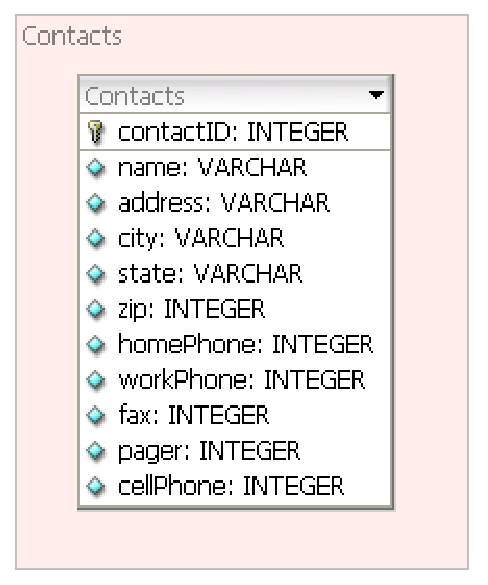
\includegraphics{Tutorials/images/BadContactModel.pdf}}
	\caption{A poorly designed contacts database}
	\label{fig:BadContactModel}
\end{figure}

\subsection{Going back and doing it right}

This program needs to store information on customers.  First, we need to define the 
customer:
\begin{quote}
A customer is any person who has done business with us or who we think might do 
business with us in the future. We need to know this person�s name, address, phone 
numbers, and email address in order to contact him or her.
\end{quote}

\subsubsection{Tackling the Name}

Ok, so we have this definition and we have the crappy model in the previous section 
that fits this definition.  At first glance putting the name in it's own field seems like 
a very good idea.  It only takes up one column so we have less data points to store 
and our SQL statements are smaller.  But what about searchability?  Let's take the 
name John Smith for example.  I, as a user can enter the name as "John Smith", 
"Smith, John", "John W. Smith", "Mr. John Smith", and "Mr. Smith, John" and they 
would all be semantically correct.  However, if I do a search and look for name being 
"John Smith", what are the chances that I am going to come back with the proper 
entry?  Slim I would say, and for database we need absolutely certainty.  The problem 
stems from us trying to lump two nibbles of information into one data field.  Suppose 
we separate the name into firstName and lastName.  Now, it doesn't matter how the 
user semantically writes names, searching for lastName="Smith" and firstName="John" 
should return the proper result each time.  The updated model is shown in Fig.
~\ref{fig:NameUpdateModel}.

\begin{figure}[ht]
	\centering
	 \scalebox{.6}{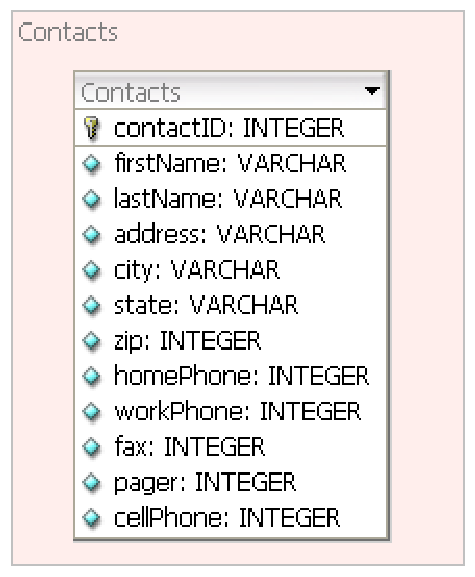
\includegraphics{Tutorials/images/NameUpdateModel.pdf}}
	\caption{Updated Name Fields}
	\label{fig:NameUpdateModel}
\end{figure}

\subsubsection{Tackling the Phone Numbers}

Next, let's look just at the phone data fields for now.  To help illustrate the problem, 
we will look at some sample rows plugged into the table.  Table 
~\ref{tbl:PhoneSampleData} shows us the data (with address info removed to 
reduce it).  Do you see anything wrong with it?  

\begin{center}
	\tablefirsthead
	{%
		\hline
		\multicolumn{1}{|c}{firstName} &
		\multicolumn{1}{|c}{lastName} &
		\multicolumn{1}{|c}{homePhone} &
		\multicolumn{1}{|c}{workPhone} &
		\multicolumn{1}{|c}{cellPhone} &
		\multicolumn{1}{|c}{fax} &
		\multicolumn{1}{c|}{pager} \\
		\hline
		\hline
	}
	
	\tablehead
	{%
		\hline
		\multicolumn{7}{|l|}{\small\sl continued from previous page}\\
		\hline
		\multicolumn{1}{|c}{firstName} &
		\multicolumn{1}{|c}{lastName} &
		\multicolumn{1}{|c}{homePhone} &
		\multicolumn{1}{|c}{workPhone} &
		\multicolumn{1}{|c}{cellPhone} &
		\multicolumn{1}{|c}{fax} &
		\multicolumn{1}{c|}{pager} \\
		\hline
		\hline
	}
	
	\tabletail
	{%
		\hline
		\multicolumn{7}{|r|}{\small\sl continued on next page}\\
		\hline
	}
	
	\tablelasttail{\hline}
	\bottomcaption{Example phone data for a bad database}
 	\label{tbl:PhoneSampleData}
	
	\begin{supertabular}{|l|l|l|l|l|l|l|}
		George & Barnes & 562-874-1234 & & 310-999-3628 & & \\ \hline
		Susan & Noble & 562-975-3388 & 714-847-3366 & & & \\ \hline
		Erwin & Star & & & & 714-997-5885 & 714-997-2428 \\ \hline
		Alice & Buck & & 562-577-1200 & 562-561-1921 & & \\ \hline
		Frank & Borders & 714-968-8201 & & & & \\ \hline
		Hanna & Diedrich & & & 562-786-7727 & & \\
	\end{supertabular}
\end{center}

There are at least two very large problems here:
\begin{itemize}
	\item There is no contact on that list that has every phone number.  The majority
		of the contacts will only have one or two numbers, which means there are a 
		lot of fields that are NULL (NULL being the constant value that means the field 
		hasn't been assigned a value).  We want to eliminate all of the unnecessary 
		NULL values in our design.
	\item Even though we provide 5 phone number fields, someone will want another 
		phone number added sooner or later.  If we want to add another phone number 
		field we actually have to change the table structure.  This is very bad design.  
		Information that colud change, like these phone numbers columns, should be kept 
		as data in a table rather than a part of the data structure.
\end{itemize}

When looking closer we realize that we don't have five single attributes.  There is 
rather a single repeated attribute, phone number.  The phone has an attribute of it's 
own telling us the type of number that it is.  This is sometimes called a weak entity, 
though it is easier to think of it as a class within a class.  So, we will pull the phone 
number out into it's own table.  I neglected to show email because it follows the same 
structure as the phone numbers.  A person can have a work email, home email, and 
more.  When the phone numbers and the emails are pulled out of the contacts table, 
we get the model shown in Fig.~\ref{fig:PhoneUpdateModel}.  As we can see, this 
already looks cleaner.

\begin{figure}[ht]
	\centering
	 \scalebox{.6}{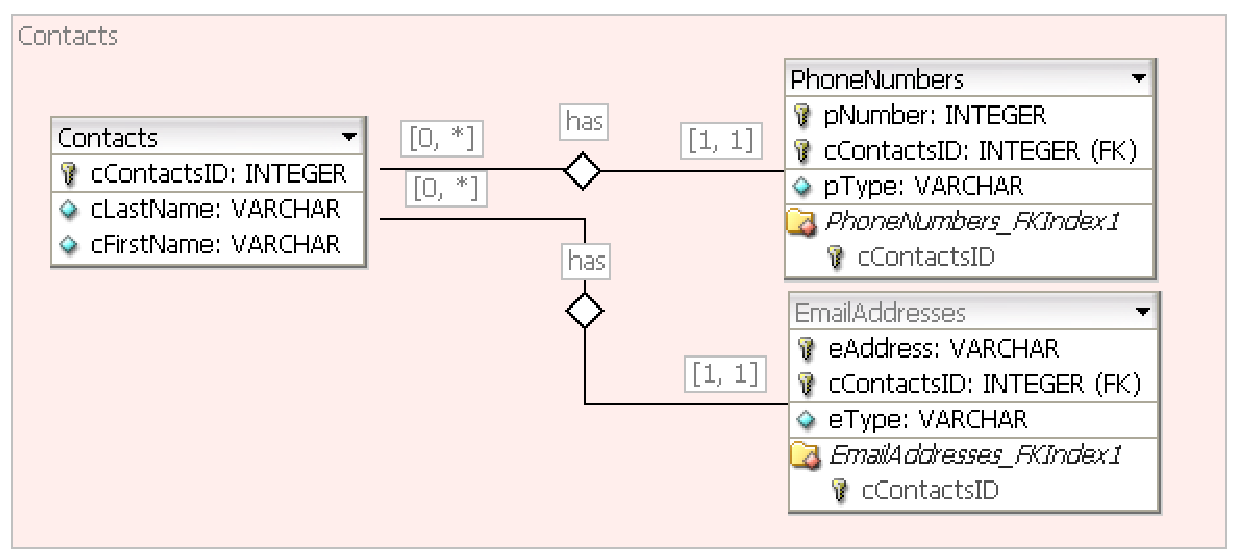
\includegraphics{Tutorials/images/PhoneUpdateModel.pdf}}
	\caption{Updated the phone fields for the contacts database}
	\label{fig:PhoneUpdateModel}
\end{figure}

\subsubsection{Tackling the Address}

Now we need to add the address fields into our database.  But should they just be 
added to the contacts table like in the previous design?  Or do they need to be 
normalized like the phone numbers and email addresses?  It's not obvious at first, but 
we need to normalize the database.  Let's look at Table~\ref{tbl:AddressSampleData} 
which shows some sample data from the contacts table with the address fields.  
Notice the repeated city and state attributes?  This is not only redundant data, but 
we also have increased potential for typos (notice the typo in row 5?).  
\begin{center}
	\tablefirsthead
	{%
		\hline
		\multicolumn{1}{|c}{firstName} &
		\multicolumn{1}{|c}{lastName} &
		\multicolumn{1}{|c}{street} &
		\multicolumn{1}{|c}{zipCode} &
		\multicolumn{1}{|c}{city} &
		\multicolumn{1}{c|}{state} \\
		\hline
		\hline
	}
	
	\tablehead
	{%
		\hline
		\multicolumn{6}{|l|}{\small\sl continued from previous page}\\
		\hline
		\multicolumn{1}{|c}{firstName} &
		\multicolumn{1}{|c}{lastName} &
		\multicolumn{1}{|c}{street} &
		\multicolumn{1}{|c}{zipCode} &
		\multicolumn{1}{|c}{city} &
		\multicolumn{1}{c|}{state} \\
		\hline
		\hline
	}
	
	\tabletail
	{%
		\hline
		\multicolumn{6}{|r|}{\small\sl continued on next page}\\
		\hline
	}
	
	\tablelasttail{\hline}
	\bottomcaption{Example phone data for a bad database}
 	\label{tbl:AddressSampleData}
	
	\begin{supertabular}{|l|l|l|l|l|l|}
		George & Barnes & 1254 Bellflower & 90840 & Long Beach & CA \\ \hline
		Susan & Noble & 1515 Palo Verde & 90840 & Long Beach & CA \\ \hline
		Erwin & Star & 17022 Brookhurst & 92708 & Fountain Valley & CA \\ \hline
		Alice & Buck & 3884 Atherton & 90836 & Long Beach & CA \\ \hline
		Frank & Borders & 10200 Slater & 92708 & Fountian Valley & CA \\ \hline
		Hanna & Diedrich & 1699 Studebaker & 90840 & Long Beach & CA \\ \hline
	\end{supertabular}
\end{center}

The problem here lies in the fact that the city and the state are functionally 
dependent on the zip code.  This means that I can uniquely determine the value of 
the city and state attributes if given a table that has data plus the value of the zip 
code.  The zip code is what is called a subkey of the Contacts table.  It is not a 
super key, but it functionally determines the city and state.  In other words, if you 
know the zip code, you can always find the city and state.  In order to solve this 
problem, we need to:
\begin{itemize}
	\item Remove all of the attributes dependent on the subkey and put them into a 
		new table called ZipLocations.
	\item Set the primary key attribute of the ZipLocations table as a duplicate of the
		subkey zipCode.
	\item Leave a copy of the zipCode attribute in the Contacts table. The zipCode 
		attribute is no longer a subkey because we moved every attribute that was 
		dependent on it into a ZipLocations table.  It now becomes a foreign key and 
		there is a many-to-one relationship between the Contacts table and the 
		ZipLocations table.
\end{itemize}

The updated database model can be seen in Fig.~\ref{fig:FinalContactModel}.

\begin{figure}[ht]
	\centering
	 \scalebox{.6}{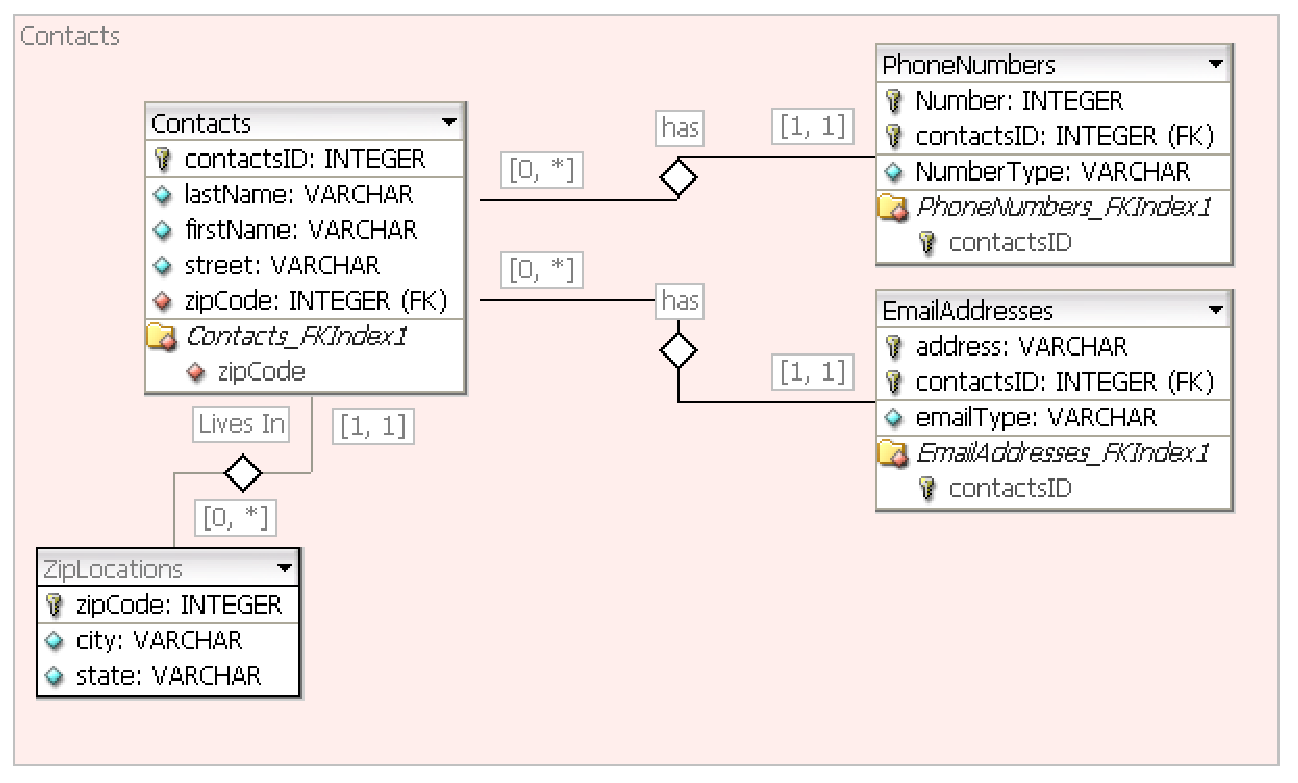
\includegraphics{Tutorials/images/FinalContactModel.pdf}}
	\caption{The Final Design For The Contacts Database}
	\label{fig:FinalContactModel}
\end{figure}

\section{Database Implementation}

Dabo supports several databases.  Dabo takes care of all of the interfacing so each 
database is can be mated plug and play with the application.  While we have several 
choices for databases we will be using a MySQL database for this program because 
it is free for non-commercial applications and available to everyone.  This book 
assumes some knowledge of setting up and administering database systems.  These 
topics will be outside the scope of this book.  There are several excellent tutorials 
out there on how to do this.

Many people think that Dabo provides framework methods to create tables and 
administer a database.  Dabo does not provide any of this functionality.  This is in 
part due to the specific nuances of SQL for different implementations and in part 
due to the abundance of database administration programs that do a spectacular 
job already.  We felt this need was more of a systems administrator job rather than 
a developer's job.  So, please set up this database and it's table before continuing 
to the next section.

\section{Backend Interfacing with Biz Objects}

By now, we hope that you have been successful setting up the MySQL database 
with the correct tables.  If not, please consult the internet for ways in which to do 
this.  We have this database, now how exactly do we interface to it?  If you remember 
from the introduction Dabo provides 3 tiers of functionality: the database layer, the 
business rules layer, and the user interface layer.  For most programs, we can 
completely ignore the database layer.

The database layer (db layer) controls all of the access to the various databases. 
It's sole functionality is to send and receive data from the database.  The good thing 
for developers that use the framework is that you can largely ignore this layer as it's
functionality is accessed through the business rules layer (biz layer).




%This section reserved for bibliography and index
\backmatter

%\include{bibliography}  % include bibliography
%\include{index}         % include index

\end{document}                          % The required last line
